\question{Câu 6}

Thiết kế một bộ sắp xếp song song như hình dưới, mô tả giải thuật sắp xếp 8 mẫu ngõ vào $x_{1}$, $x_{2}$,$\dots, x_{8}$, và cho ngõ ra là $y_{1}$, $y_{2}$, $\dots, y_{8}$ theo thứ tự giảm dần (hoặc tăng dần).

\begin{figure}[H]
	\centering
	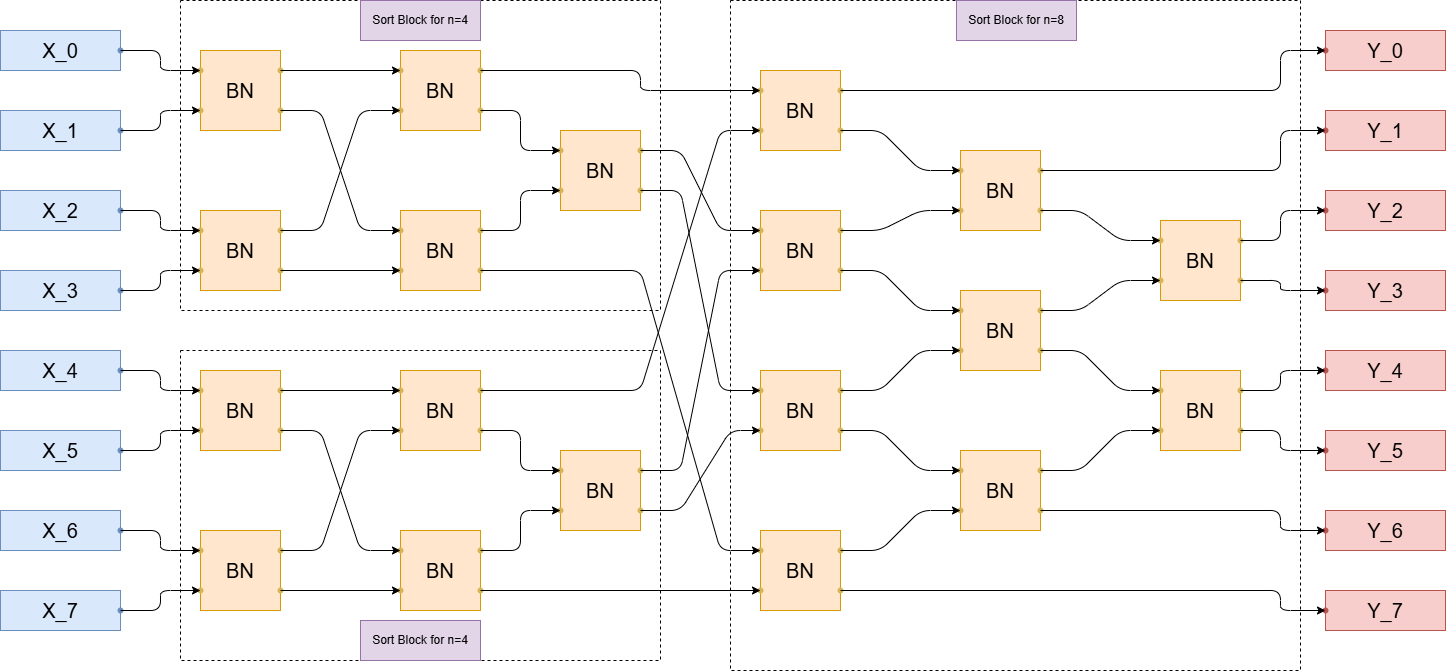
\includegraphics[width=\linewidth]{./my-chapters/my-diagrams/Question6/debai.png}
\end{figure}

Trong đó, mỗi bộ BN (Bitonic Merger Sort) có cấu trúc như hình:

\begin{figure}[H]
	\centering
	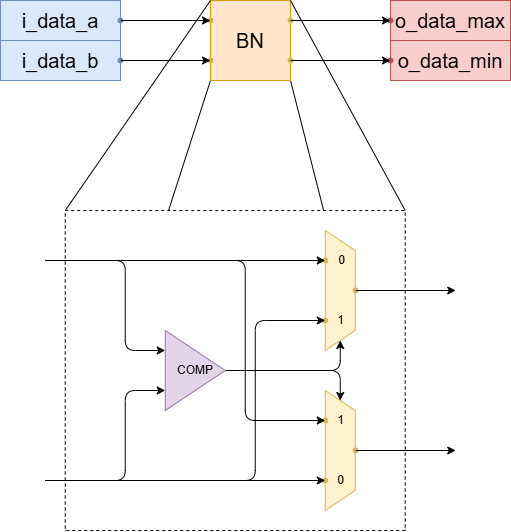
\includegraphics[width=.4\linewidth]{./my-chapters/my-diagrams/Question6/Swap_and_compare.png}
\end{figure}

Cho các standard cell là: Cổng NOT, các cổng logic 2 ngõ vào, Mux 2-1, Mux 4-1.

\answer{a}{Giả sử các mẫu ngõ vào có độ rộng là 8bit. Thiết kế mạch trên theo phương pháp đã cho và chỉ được sử dụng các standard cell trên.}

\begin{itemize}[label=-]
	\item \textbf{Bộ so sánh 8bit}
	
	\begin{itemize}[label=+]
		\item Triển khai bộ so sánh 2-bit
		
		\begin{table}[H]
			\centering
			\begin{tabular}{|c|c|c|c|c|c|}
				\hline 
				\multicolumn{4}{|c|}{Input} & \multicolumn{2}{c|}{Output}\\
				\hline
				$ a_{1} $ & $ a_{0} $ & $ b_{1} $ & $ b_{0} $ & less & equal \\
				\hline
				0 & 0 & 0 & 0 & 0 & 1\\
				\hline
				0 & 0 & 0 & 1 & 1 & 0\\
				\hline
				0 & 0 & 1 & 0 & 1 & 0\\
				\hline
				0 & 0 & 1 & 1 & 1 & 0\\
				\hline
				0 & 1 & 0 & 0 & 0 & 0\\
				\hline
				0 & 1 & 0 & 1 & 0 & 1\\
				\hline
				0 & 1 & 1 & 0 & 1 & 0\\
				\hline
				0 & 1 & 1 & 1 & 1 & 0\\
				\hline
				1 & 0 & 0 & 0 & 0 & 0\\
				\hline
				1 & 0 & 0 & 1 & 0 & 0\\
				\hline
				1 & 0 & 1 & 0 & 0 & 1\\
				\hline
				1 & 0 & 1 & 1 & 0 & 0\\
				\hline
				1 & 1 & 0 & 0 & 0 & 0\\
				\hline
				1 & 1 & 0 & 1 & 0 & 0\\
				\hline
				1 & 1 & 1 & 0 & 0 & 0\\
				\hline
				1 & 1 & 1 & 1 & 0 & 1\\
				\hline
			\end{tabular}
			\caption{Bảng sự thật cho bộ so sánh 2-bit $ A \,<\, B $.}
			\label{tab: comparator 2bit}
		\end{table}
	
		Từ bộ bảng sự thật \ref{tab: comparator 2bit}, ta rút gọn kìa K về dạng như sau:
		
		\begin{figure}[H]
			\centering
			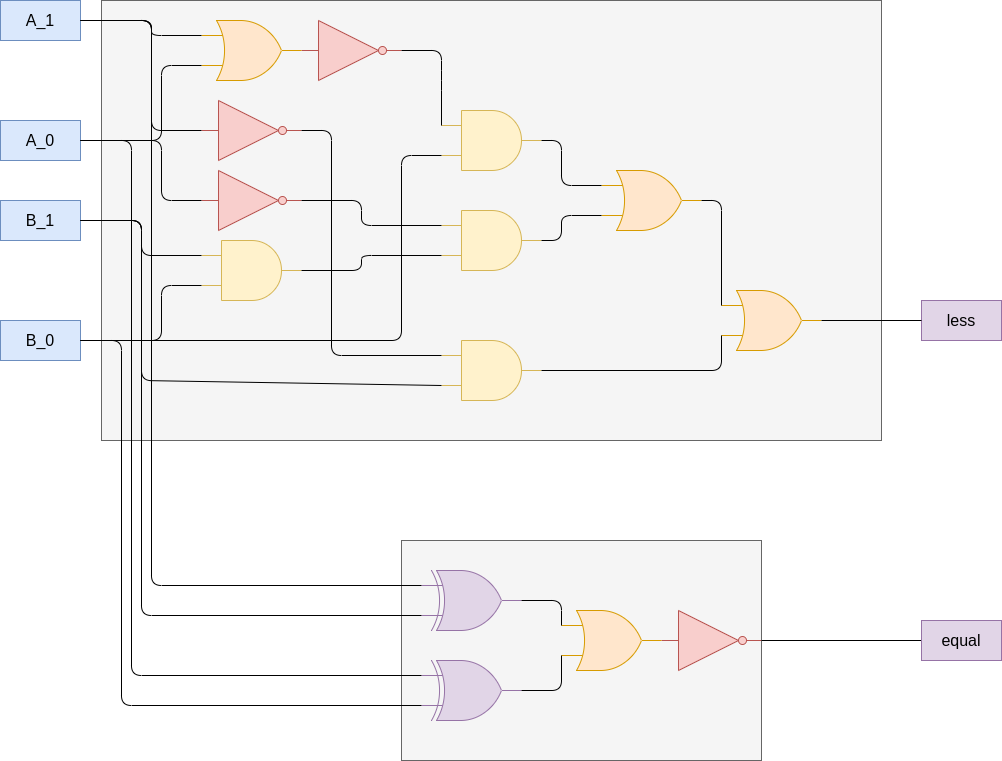
\includegraphics[width=.9\linewidth]{./my-chapters/my-diagrams/Question6/comparator_2bit.png}
			\caption{Sơ đồ logic của bộ Comparator 2-bit.}
		\end{figure}
	
		\item Triển khai bộ so sánh 4-bit
		
		\begin{minipage}{.4\linewidth}
			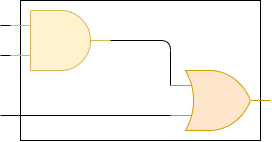
\includegraphics[width=.7\linewidth]{./my-chapters/my-diagrams/Question6/propagation.png}
		\end{minipage}
		\begin{minipage}{.4\linewidth}
			Sử dụng bộ lan truyền dấu so sánh trên, với nếu các bit trên có có xuất hiện bit less thì ngõ ra lan truyền bit less, còn nếu bit thấp thì nếu tầng trên bằng nhau và các tầng thấp có bit less ngõ ra lan truyền bit less.
		\end{minipage}
		
		\begin{figure}[H]
			\centering
			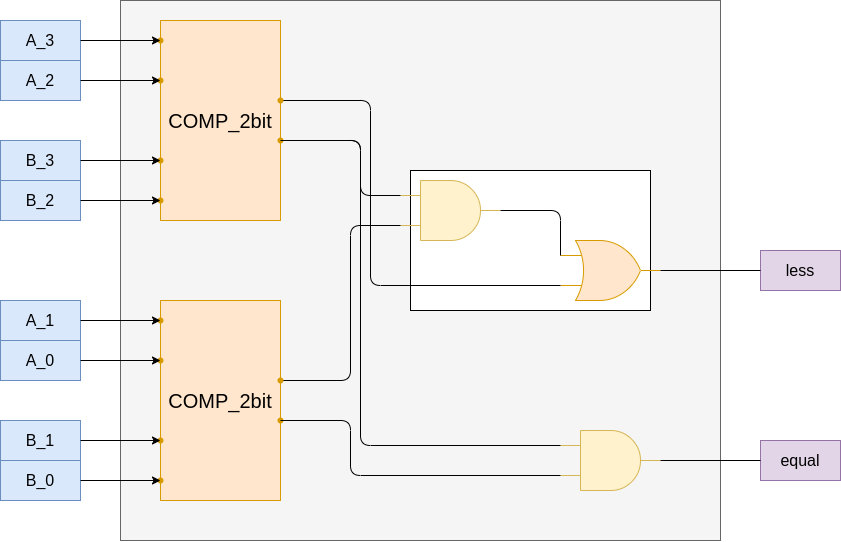
\includegraphics[width=.9\linewidth]{./my-chapters/my-diagrams/Question6/comparator_4bit.png}
			\caption{Sơ đồ logic của bộ Comparator 4-bit.}
		\end{figure}
	
		\item Triển khai bộ so sánh 8-bit
		
		Tương tự với bộ 4-bit, thì 8-bit được triển khai với 2 bộ 4-bit.
		
		\begin{figure}[H]
			\centering
			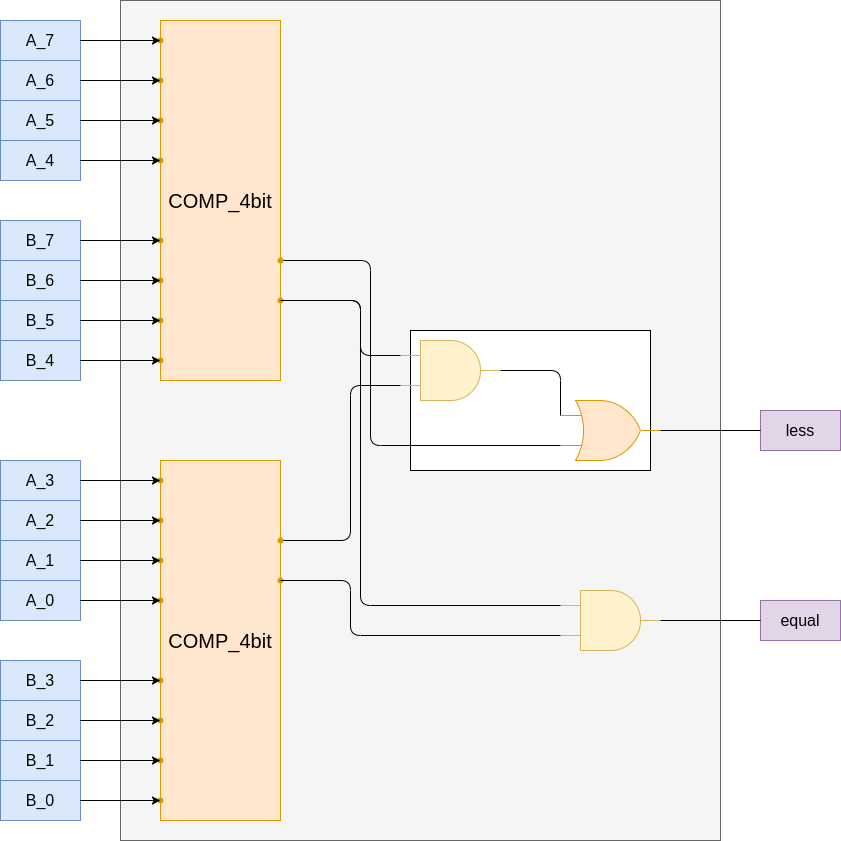
\includegraphics[width=.9\linewidth]{./my-chapters/my-diagrams/Question6/comparator_8bit.png}
			\caption{Sơ đồ logic của bộ Comparator 8-bit.}
		\end{figure}
	\end{itemize}

	\item \textbf{Bộ Swap 8bit}
	
	\begin{figure}[H]
		\centering
		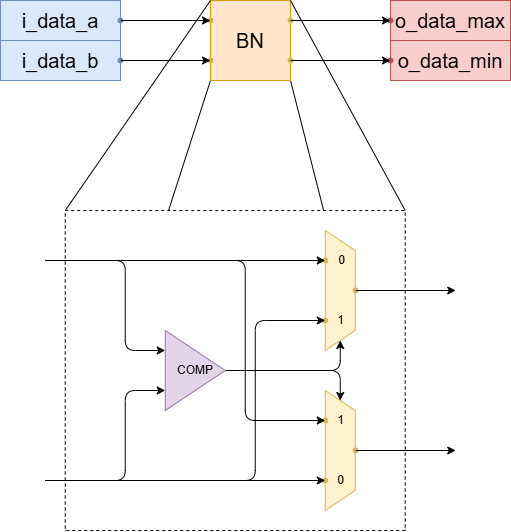
\includegraphics[width=.4\linewidth]{./my-chapters/my-diagrams/Question6/Swap_and_compare.png}
		\caption{Bộ so sánh và swap giá trị trong Bitonic Merger Sort.}
	\end{figure}

	\item \textbf{Bitonic Merger Sort}
	
	\begin{figure}[H]
		\centering
		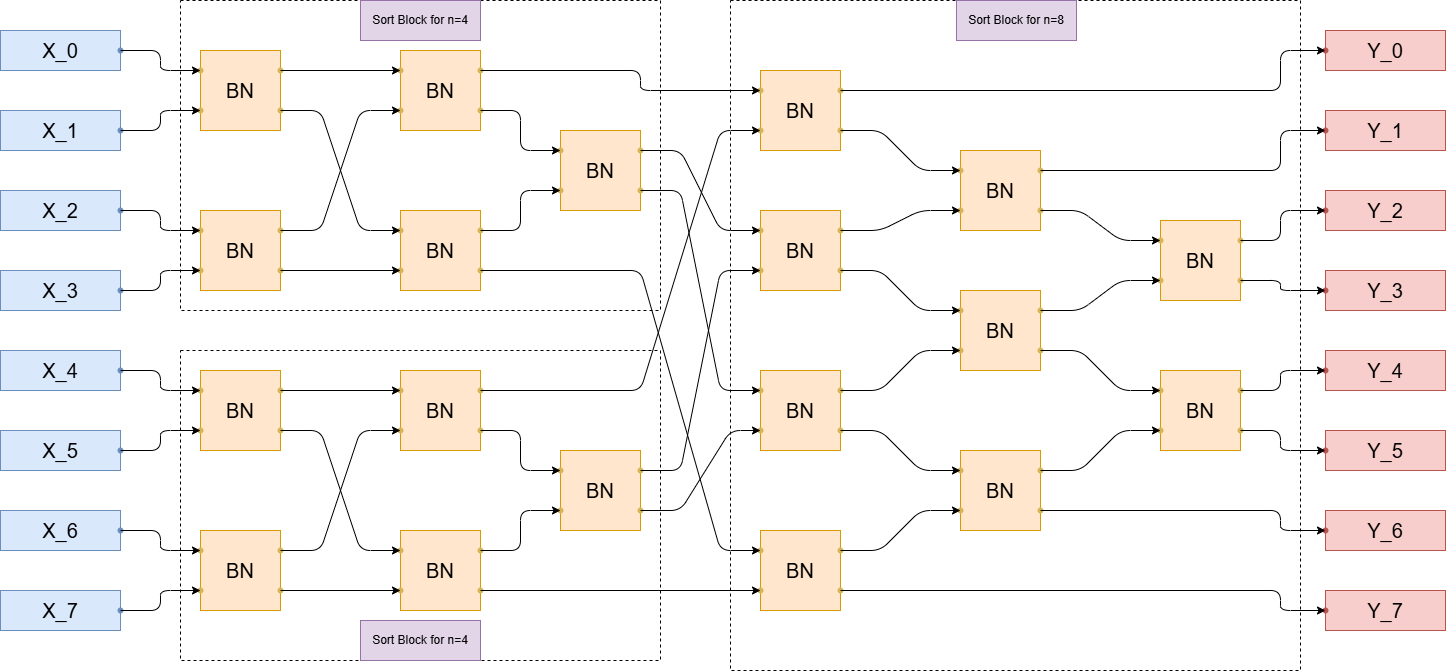
\includegraphics[width=\linewidth]{./my-chapters/my-diagrams/Question6/debai.png}
		\caption{Bộ sắp xếp Bitonic Merger Sort.}
	\end{figure}
\end{itemize}

\answer{b}{Viết chương trình HDL mô tả mạch đã cho.}

\lstinputlisting[style=StyleCode, language=SystemVerilog, caption={Chương trình mô tả bộ so sánh 2-bit.}]{./../02_rtl/Question6/COMP_2bit.sv}

\lstinputlisting[style=StyleCode, language=SystemVerilog, caption={Chương trình mô tả bộ so sánh 4-bit.}]{./../02_rtl/Question6/COMP_4bit.sv}

\lstinputlisting[style=StyleCode, language=SystemVerilog, caption={Chương trình mô tả bộ so sánh 8-bit.}]{./../02_rtl/Question6/COMP_less.sv}

\lstinputlisting[style=StyleCode, language=SystemVerilog, caption={Chương trình mô tả một đơn vị của bộ Bitonic Merger Sort.}]{./../02_rtl/Question6/Compare_and_Swap_unit.sv}

\lstinputlisting[style=StyleCode, language=SystemVerilog, caption={Chương trình mô tả bộ Bitonic Merger Sort Block-4.}]{./../02_rtl/Question6/Bitonic_Block4.sv}

\lstinputlisting[style=StyleCode, language=SystemVerilog, caption={Chương trình mô tả bộ Bitonic Merger Sort Block-8.}]{./../02_rtl/Question6/Bitonic_Block8.sv}

\lstinputlisting[style=StyleCode, language=SystemVerilog, caption={Chương trình mô tả bộ Bitonic Merger Sort 8 phần tử đầu vào.}]{./../02_rtl/Question6/Bitonic_Sort.sv}

\answer{c}{Viết chương trình testbench cho mạch.}

Đầu tiên nhóm em thực hiện triển khai chứng minh giải thuật kết quả đúng của bài toán sau:

\begin{lstlisting}[style=StyleCode, language=SystemVerilog, caption={Giải thuật chứng minh bộ Bitonic Merger Sort 8 phần tử.}]
	function automatic logic [SIZE_DATA*NUM_ELEM-1:0] f_ARR_sorted(
		int                                  f_is_acs   ,
		input logic [SIZE_DATA*NUM_ELEM-1:0] f_i_data
	);
		logic [SIZE_DATA-1:0] arr   [0:NUM_ELEM-1];
		logic [SIZE_DATA-1:0] temp;
		int i, j;
	
		begin
			for (i = 0; i < NUM_ELEM; i++) begin
				arr[i] = f_i_data[i*SIZE_DATA +: SIZE_DATA];
			end
			
			for (i = 0; i < NUM_ELEM-1; i++) begin
				for (j = 0; j < NUM_ELEM-1-i; j++) begin
					if(f_is_acs) begin
						if (arr[j] > arr[j+1]) begin
							temp     = arr[j];
							arr[j]   = arr[j+1];
							arr[j+1] = temp;
						end 
					end else begin
						if (arr[j] < arr[j+1]) begin
							temp     = arr[j];
							arr[j]   = arr[j+1];
							arr[j+1] = temp;
						end
					end
				end
			end
	
		for (i = 0; i < NUM_ELEM; i++) begin
			f_ARR_sorted[i*SIZE_DATA +: SIZE_DATA] = arr[i];
		end
	end
	endfunction
\end{lstlisting}

Nhóm em sử dụng giải thuật của Bubble Sort gần giống với giải thuật parallel của Bitonic Merger Sort, và một task để hiển thị kêt quả một các trực quan.

\begin{lstlisting}[style=StyleCode, language=SystemVerilog]
	task automatic Display_Result(
		string                               t_type,
		input logic [SIZE_DATA*NUM_ELEM-1:0] t_arr
		);
		logic [SIZE_DATA-1:0] t_t_arr   [0:NUM_ELEM-1];
		int i, j;
			begin
			for (i = 0; i < NUM_ELEM; i++) begin
				t_t_arr[i] = t_arr[i*SIZE_DATA +: SIZE_DATA];
			end
			
			for (j = 0; j < NUM_ELEM; j++) begin
				$display("%s[%d] \t= %8h (%d)", t_type, j, t_t_arr[j], t_t_arr[j]);
			end
			end
	endtask //automatic
\end{lstlisting}
{\centering\textbf{Thực hiện với bộ sắp xếp tăng dần}}
\begin{itemize}[label=-]
	\item TestCase0: Thực hiện test với 8 phần tử đầu vào đều là \textsf{8'b0}.
	\begin{lstlisting}[style=StyleCode, language=SystemVerilog, caption={Test trường hợp các đầu vào đều là không.}]
		repeat (1) begin
			@(posedge i_clk);
			#1;
			i_data  = $urandom;
			i_data = '0;
			$display("\n");
			Display_Result("Input", i_data);
			@(negedge i_clk);
			#1;
			$display("\n");
			Display_Result("Output", o_data);
			$display("[TIME: %5t] [%s] i_data = %h (%d) \t| o_data = %h (%d)", $time, "Zero", i_data, i_data, o_data, o_data);
			$display("=> %4s: Expect: %8h, DUT: %8h ", (f_ARR_sorted(IS_ASC, i_data) == o_data) ? "PASS" : "FAIL", f_ARR_sorted(IS_ASC, i_data), o_data);
			test_count = test_count + 1;
			test_pass  = (f_ARR_sorted(IS_ASC, i_data) == o_data) ? test_pass + 1 : test_pass;
		end
	\end{lstlisting}

	Kết quả
	
	\begin{lstlisting}[style=StyleResult, language=Result, caption={Kết quả khi cho 8 phần tử ngõ vào đều là không.}]
		===ACSENDING===

		Input[          0] 	= 00000000 (  0)
		Input[          1] 	= 00000000 (  0)
		Input[          2] 	= 00000000 (  0)
		Input[          3] 	= 00000000 (  0)
		Input[          4] 	= 00000000 (  0)
		Input[          5] 	= 00000000 (  0)
		Input[          6] 	= 00000000 (  0)
		Input[          7] 	= 00000000 (  0)
		
		Output[          0] 	= 00000000 (  0)
		Output[          1] 	= 00000000 (  0)
		Output[          2] 	= 00000000 (  0)
		Output[          3] 	= 00000000 (  0)
		Output[          4] 	= 00000000 (  0)
		Output[          5] 	= 00000000 (  0)
		Output[          6] 	= 00000000 (  0)
		Output[          7] 	= 00000000 (  0)
		[TIME: 41000] [Zero] i_data = 0000000000000000 (                   0) 	| o_data = 0000000000000000 (                   0)
		=> PASS: Expect: 00000000, DUT: 00000000 
	\end{lstlisting}

	\item Testcase1: Thực hiện và hiển thị một trường hợp để kiểm tra các hoạt động.
	
	\begin{lstlisting}[style=StyleCode, language=SystemVerilog, caption={Test 1 trường hợp ngầu nhiên.}]
		repeat (1) begin
			@(posedge i_clk);
			#1;
			i_data  = $urandom;
			$display("\n");
			Display_Result("Input", i_data);
			@(negedge i_clk);
			#1;
			$display("\n");
			Display_Result("Output", o_data);
			$display("[TIME: %5t] [%s] i_data = %h (%d) \t| o_data = %h (%d)", $time, "Random", i_data, i_data, o_data, o_data);
			$display("=> %4s: Expect: %8h, DUT: %8h ", (f_ARR_sorted(IS_ASC, i_data) == o_data) ? "PASS" : "FAIL", f_ARR_sorted(IS_ASC, i_data), o_data);
			test_count = test_count + 1;
			test_pass  = (f_ARR_sorted(IS_ASC, i_data) == o_data) ? test_pass + 1 : test_pass;
		end
	\end{lstlisting}
	
	Kết quả
	
	\begin{lstlisting}[style=StyleResult, language=Result, caption={Kết quả khi cho 1 trường hợp ngầu nhiên.}]
		===ACSENDING===
		
		Input[          0] 	= 0000009c (156)
		Input[          1] 	= 0000005d ( 93)
		Input[          2] 	= 0000001e ( 30)
		Input[          3] 	= 0000000b ( 11)
		Input[          4] 	= 00000000 (  0)
		Input[          5] 	= 00000000 (  0)
		Input[          6] 	= 00000000 (  0)
		Input[          7] 	= 00000000 (  0)
		
		
		Output[          0] 	= 00000000 (  0)
		Output[          1] 	= 00000000 (  0)
		Output[          2] 	= 00000000 (  0)
		Output[          3] 	= 00000000 (  0)
		Output[          4] 	= 0000000b ( 11)
		Output[          5] 	= 0000001e ( 30)
		Output[          6] 	= 0000005d ( 93)
		Output[          7] 	= 0000009c (156)
		[TIME: 51000] [Random] i_data = 000000000b1e5d9c (           186539420) 	| o_data = 9c5d1e0b00000000 (11267194875344322560)
		=> PASS: Expect: 9c5d1e0b00000000, DUT: 9c5d1e0b00000000 
	\end{lstlisting}

	\item Testcase1: Thực hiện và 100 trường hợp để kiểm tra các hoạt động.
	
	\begin{lstlisting}[style=StyleCode, language=SystemVerilog, caption={Test 100 trường hợp ngầu nhiên.}]
		repeat (100) begin
			@(posedge i_clk);
			#1;
			i_data  = $urandom_range(0, 2**(SIZE_DATA*NUM_ELEM)-1);
			@(negedge i_clk);
			#1;
			$display("[TIME: %5t] [%s] i_data = %h (%d) \t| o_data = %h (%d)", $time, "Random", i_data, i_data, o_data, o_data);
			$display("=> %4s: Expect: %8h, DUT: %8h ", (f_ARR_sorted(IS_ASC, i_data) == o_data) ? "PASS" : "FAIL", f_ARR_sorted(IS_ASC, i_data), o_data);
			test_count = test_count + 1;
			test_pass  = (f_ARR_sorted(IS_ASC, i_data) == o_data) ? test_pass + 1 : test_pass;
		end
	\end{lstlisting}
	
	Kết quả
	
	\begin{lstlisting}[style=StyleResult, language=Result, caption={Kết quả khi cho 100 trường hợp ngầu nhiên.}]
		===ACSENDING===
		
		[TIME: 61000] [Random] i_data = 000000009efdd502 (          2667435266) 	| o_data = fdd59e0200000000 (18290699193062260736)
		=> PASS: Expect: fdd59e0200000000, DUT: fdd59e0200000000 
		[TIME: 71000] [Random] i_data = 0000000048c2e0e4 (          1220731108) 	| o_data = e4e0c24800000000 (16492395449924190208)
		=> PASS: Expect: e4e0c24800000000, DUT: e4e0c24800000000 
		[TIME: 81000] [Random] i_data = 0000000092178378 (          2451014520) 	| o_data = 9283781700000000 (10557413991666155520)
		=> PASS: Expect: 9283781700000000, DUT: 9283781700000000 
		[TIME: 91000] [Random] i_data = 00000000bbd58ebc (          3151335100) 	| o_data = d5bcbb8e00000000 (15401391044260003840)
		=> PASS: Expect: d5bcbb8e00000000, DUT: d5bcbb8e00000000 
		...
		[TIME: 1031000] [Random] i_data = 0000000011dab302 (           299545346) 	| o_data = dab3110200000000 (15758958221387104256)
		=> PASS: Expect: dab3110200000000, DUT: dab3110200000000 
		[TIME: 1041000] [Random] i_data = 00000000ca972bfb (          3398904827) 	| o_data = fbca972b00000000 (18143480259754852352)
		=> PASS: Expect: fbca972b00000000, DUT: fbca972b00000000 
		[TIME: 1051000] [Random] i_data = 000000009f2015e8 (          2669680104) 	| o_data = e89f201500000000 (16762151612662677504)
		=> PASS: Expect: e89f201500000000, DUT: e89f201500000000 
	\end{lstlisting}

	\item Kết quả tổng kết.
	
	\begin{lstlisting}[style=StyleResult, language=SystemVerilog, caption={Kết quả của tổng kết của bài test.}]
		================================
		==========TEST SUMMARY==========
		Total test cases:    102    
		Passed          :    102    
		Failed          :      0    
		Pass rate       : 100.00%
		================================
		
	\end{lstlisting}
\end{itemize}

{\centering\textbf{Thực hiện với bộ sắp xếp giảm dần}}
\begin{itemize}[label=-]
	\item TestCase0: Thực hiện test với 8 phần tử đầu vào đều là \textsf{8'b0}.
%	\begin{lstlisting}[style=StyleCode, language=SystemVerilog, caption={Test trường hợp các đầu vào đều là không.}]
%		repeat (1) begin
%		@(posedge i_clk);
%		#1;
%		i_data  = $urandom;
%		i_data = '0;
%		$display("\n");
%		Display_Result("Input", i_data);
%		@(negedge i_clk);
%		#1;
%		$display("\n");
%		Display_Result("Output", o_data);
%		$display("[TIME: %5t] [%s] i_data = %h (%d) \t| o_data = %h (%d)", $time, "Zero", i_data, i_data, o_data, o_data);
%		$display("=> %4s: Expect: %8h, DUT: %8h ", (f_ARR_sorted(IS_ASC, i_data) == o_data) ? "PASS" : "FAIL", f_ARR_sorted(IS_ASC, i_data), o_data);
%		test_count = test_count + 1;
%		test_pass  = (f_ARR_sorted(IS_ASC, i_data) == o_data) ? test_pass + 1 : test_pass;
%		end
%	\end{lstlisting}
%	
%	Kết quả
%	
	\begin{lstlisting}[style=StyleResult, language=Result, caption={Kết quả khi cho 8 phần tử ngõ vào đều là không.}]
		===DESCENDING===
		
		Input[          0] 	= 00000000 (  0)
		Input[          1] 	= 00000000 (  0)
		Input[          2] 	= 00000000 (  0)
		Input[          3] 	= 00000000 (  0)
		Input[          4] 	= 00000000 (  0)
		Input[          5] 	= 00000000 (  0)
		Input[          6] 	= 00000000 (  0)
		Input[          7] 	= 00000000 (  0)
		
		
		Output[          0] 	= 00000000 (  0)
		Output[          1] 	= 00000000 (  0)
		Output[          2] 	= 00000000 (  0)
		Output[          3] 	= 00000000 (  0)
		Output[          4] 	= 00000000 (  0)
		Output[          5] 	= 00000000 (  0)
		Output[          6] 	= 00000000 (  0)
		Output[          7] 	= 00000000 (  0)
		[TIME: 41000] [Zero] i_data = 0000000000000000 (                   0) 	| o_data = 0000000000000000 (                   0)
		=> PASS: Expect: 00000000, DUT: 00000000 
	\end{lstlisting}
	
	\item Testcase1: Thực hiện và hiển thị một trường hợp để kiểm tra các hoạt động.
	
%	\begin{lstlisting}[style=StyleCode, language=SystemVerilog, caption={Test 1 trường hợp ngầu nhiên.}]
%		repeat (1) begin
%		@(posedge i_clk);
%		#1;
%		i_data  = $urandom;
%		$display("\n");
%		Display_Result("Input", i_data);
%		@(negedge i_clk);
%		#1;
%		$display("\n");
%		Display_Result("Output", o_data);
%		$display("[TIME: %5t] [%s] i_data = %h (%d) \t| o_data = %h (%d)", $time, "Random", i_data, i_data, o_data, o_data);
%		$display("=> %4s: Expect: %8h, DUT: %8h ", (f_ARR_sorted(IS_ASC, i_data) == o_data) ? "PASS" : "FAIL", f_ARR_sorted(IS_ASC, i_data), o_data);
%		test_count = test_count + 1;
%		test_pass  = (f_ARR_sorted(IS_ASC, i_data) == o_data) ? test_pass + 1 : test_pass;
%		end
%	\end{lstlisting}
%	
%	Kết quả
%	
	\begin{lstlisting}[style=StyleResult, language=Result, caption={Kết quả khi cho 1 trường hợp ngầu nhiên.}]
		===DESCENDING===
		
		Input[          0] 	= 0000009c (156)
		Input[          1] 	= 0000005d ( 93)
		Input[          2] 	= 0000001e ( 30)
		Input[          3] 	= 0000000b ( 11)
		Input[          4] 	= 00000000 (  0)
		Input[          5] 	= 00000000 (  0)
		Input[          6] 	= 00000000 (  0)
		Input[          7] 	= 00000000 (  0)
		
		
		Output[          0] 	= 0000009c (156)
		Output[          1] 	= 0000005d ( 93)
		Output[          2] 	= 0000001e ( 30)
		Output[          3] 	= 0000000b ( 11)
		Output[          4] 	= 00000000 (  0)
		Output[          5] 	= 00000000 (  0)
		Output[          6] 	= 00000000 (  0)
		Output[          7] 	= 00000000 (  0)
		[TIME: 51000] [Random] i_data = 000000000b1e5d9c (           186539420) 	| o_data = 000000000b1e5d9c (           186539420)
		=> PASS: Expect: 0b1e5d9c, DUT: 0b1e5d9c 
	\end{lstlisting}
	
	\item Testcase1: Thực hiện và 100 trường hợp để kiểm tra các hoạt động.
	
%	\begin{lstlisting}[style=StyleCode, language=SystemVerilog, caption={Test 100 trường hợp ngầu nhiên.}]
%		repeat (100) begin
%		@(posedge i_clk);
%		#1;
%		i_data  = $urandom_range(0, 2**(SIZE_DATA*NUM_ELEM)-1);
%		@(negedge i_clk);
%		#1;
%		$display("[TIME: %5t] [%s] i_data = %h (%d) \t| o_data = %h (%d)", $time, "Random", i_data, i_data, o_data, o_data);
%		$display("=> %4s: Expect: %8h, DUT: %8h ", (f_ARR_sorted(IS_ASC, i_data) == o_data) ? "PASS" : "FAIL", f_ARR_sorted(IS_ASC, i_data), o_data);
%		test_count = test_count + 1;
%		test_pass  = (f_ARR_sorted(IS_ASC, i_data) == o_data) ? test_pass + 1 : test_pass;
%		end
%	\end{lstlisting}
%	
%	Kết quả
%	
	\begin{lstlisting}[style=StyleResult, language=Result, caption={Kết quả khi cho 100 trường hợp ngầu nhiên.}]
		===DESCENDING===
		
		[TIME: 61000] [Random] i_data = 000000009efdd502 (          2667435266) 	| o_data = 00000000029ed5fd (            43963901)
		=> PASS: Expect: 029ed5fd, DUT: 029ed5fd 
		[TIME: 71000] [Random] i_data = 0000000048c2e0e4 (          1220731108) 	| o_data = 0000000048c2e0e4 (          1220731108)
		=> PASS: Expect: 48c2e0e4, DUT: 48c2e0e4 
		[TIME: 81000] [Random] i_data = 0000000092178378 (          2451014520) 	| o_data = 0000000017788392 (           393773970)
		=> PASS: Expect: 17788392, DUT: 17788392 
		...
		[TIME: 1031000] [Random] i_data = 0000000011dab302 (           299545346) 	| o_data = 000000000211b3da (            34714586)
		=> PASS: Expect: 0211b3da, DUT: 0211b3da 
		[TIME: 1041000] [Random] i_data = 00000000ca972bfb (          3398904827) 	| o_data = 000000002b97cafb (           731368187)
		=> PASS: Expect: 2b97cafb, DUT: 2b97cafb 
		[TIME: 1051000] [Random] i_data = 000000009f2015e8 (          2669680104) 	| o_data = 0000000015209fe8 (           354459624)
		=> PASS: Expect: 15209fe8, DUT: 15209fe8 
	\end{lstlisting}
	
	\item Kết quả tổng kết.
	
	\begin{lstlisting}[style=StyleResult, language=SystemVerilog, caption={Kết quả của tổng kết của bài test.}]
		================================
		==========TEST SUMMARY==========
		Total test cases:    102    
		Passed          :    102    
		Failed          :      0    
		Pass rate       : 100.00%
		================================
		
	\end{lstlisting}
\end{itemize}